%!TEX root = tesis.tex
\chapter{Aprendizaje en un \ssolver paralelo y distribuido}
\label{aprendizaje-pardist}

En el Cap.~\ref{ssolver-pardist} vimos que el enfoque de distribución aplicado
consigue disminuir el tiempo necesario para resolver una serie de problemas de
tamaño considerable. Al mismo tiempo observamos que existen casos en los que
la eficiencia --entendida como cuánto ganamos por cada unidad de \hard
agregada al cómputo de un problema-- resulta pobre. Planteamos como hipótesis
que esta situación se debe, en gran medida, a una importante cantidad de
retrabajo que se produce como consecuencia del particionado de un problema en
diversos subproblemas. 

La existencia de retrabajo se evidencia en que si bien al partir un problema
en subproblemas, el subproblema más grande suele ser más chico que el padre,
la suma del tiempo requerido para resolver todos los subproblemas hijos es
considerablemente mayor que el tiempo requerido para resolver el problema
padre. Debido al esquema de particionado recursivo, este incremento en el
tiempo total de cómputo requerido para resolver un problema se vuelve
sustancial.

En el presente capítulo desarrollaremos un mecanismo de reutilización del
conocimiento adquirido durante la ejecución de cada subproblema. Este
mecanismo persigue dos objetivos principales: verificar la hipótesis planteada
y, de ser posible,  disminuir los tiempos requeridos para resolver un problema
aumentando la eficiencia de la herramienta.

\section{Justificación del enfoque}

El enfoque de particionamiento recursivo, basado en \emph{guiding paths}, que
hemos adoptado para la construcción de la herramienta también influye en la
elección de un mecanismo adecuado para compartir información de cláusulas
aprendidas. 

\newcommand{\roottask}{\ensuremath{<\varphi_R, \emptyset>}\xspace}
\newcommand{\task}{\ensuremath{<\varphi, \emptyset>}\xspace}
\newcommand{\nonemptytask}{\ensuremath{<\varphi, C>}\xspace}

Consideremos ahora que un problema no es ya únicamente una fórmula $\varphi$
sino una tupla $<\varphi, C>$ donde $C$ es un conjunto de cláusulas tales que
$(\forall v) (v \models \varphi \Longleftrightarrow v \models \varphi
\bigwedge C)$ llamado conjunto de cláusulas aprendidas. En este contexto el
problema original es la tupla \roottask donde $\varphi_R$ denota la fórmula
original que se desea verificar. En este modelo, al partir un problema \task
levantando (por ejemplo) la variable $u$ obtenemos dos nuevos subproblemas
$<\varphi_u, \emptyset>$ y $<\varphi_{-u}, \emptyset>$. 

Notemos entonces que dado un problema \nonemptytask podemos generar los
subproblemas que resultan de levantar la variable $u$ como sigue:
$t_u=<\varphi_u, C_u>$ y $t_{-u}=<\varphi_{-u}, C_{-u}>$ (donde $C_u$ es el
conjunto de cláusulas que resulta de reemplazar las apariciones de la variable
$u$ por el valor $1$ en el conjunto $C$ y $C_{-u}$ es el resultado de
reemplazar las apariciones de la variable $u$ por el valor $0$) sin alterar la
corrección de la herramienta. Esto se debe a que si $v \models \varphi_u$
entonces $v\cup\{u\leftarrow1\} \models \varphi$ y por lo tanto
$v\cup\{u\leftarrow1\} \models \varphi \bigwedge C$ de lo que se deduce que $v
\models \varphi_u \bigwedge C_u$. Lo mismo vale para el caso $\varphi_{-u}$.

Más aún, lo antedicho vale también para cualquier subconjunto de $C$. Esto
induce una manera \emph{natural} de reutilización de las cláusulas aprendidas
que llamaremos \emph{herencia}. Este mecanismo consiste en que, al generar
nuevos subproblemas a partir de un problema padre \nonemptytask, los
subproblemas hijos son generados con un subconjunto de $C$ como conjunto de
cláusulas aprendidas. Llamaremos \emph{criterio} a cada forma distinta de
obtener un subconjunto a partir de un conjunto de cláusulas $C$.


\subsubsection{Consideraciones de escalabilidad}

Más allá de la naturalidad del enfoque inducido por el esquema de
particionado, nos interesa también evitar cualquier método que introduzca
nuevos cuellos de botella en la arquitectura. Por ejemplo, no sería aceptable
la incorporación de una gran base de datos centralizada en la que todos los
\ws almacenen las cláusulas que van aprendiendo y que todos los \ws deban
consultar.

Tampoco sería aceptable un grafo completo de comunicación permanente para
lograr ese mismo fin, es decir, hacer que cada \w le comunique (o consulte) a
todos los demás las cláusulas que va(n) aprendiendo.


\subsubsection{Independencia del \ssolver particular utilizado}

Por otro lado, como ya hemos señalado en el Cap.~\ref{ssolver-pardist}, nos
interesa que el \ssolver secuencial que utiliza cada uno de los \ws sea fácil
de actualizar y/o de reemplazar por otro componente \ots similar. Si bien
suelen ser necesarios algunos cambios para lograr que un \ssolver permita la
inyección \emph{inicial} de cláusulas aprendidas (en lugar de comenzar sin
ninguna), por lo general tales cambios se reducen a cuestiones de interfaz y
no revisten mayor dificultad.

Es más ambicioso, en cambio, pretender poder inyectar nuevas cláusulas
aprendidas en cualquier momento \emph{durante} el proceso de búsqueda. Para
ello habría que introducir modificaciones mucho más fuertemente acopladas a la
versión particular de \ssolver en uso, sus algoritmos, estructuras de datos e
invariantes particulares.

\

Es por estos factores que optamos por implementar un esquema de reutilización
de cláusulas aprendidas basado en herencia. En esencia el esquema funciona de
acuerdo a lo detallado al comienzo de esta sección. En particular, a la hora
de partir un problema en nuevos subproblemas un \emph{criterio} es aplicado al
conjunto de cláusulas aprendidas que el problema padre poseía al momento de
ser abortado. De esta manera se generan los subconjuntos de cláusulas
aprendidas que los subproblemas hijos deberán incorporar antes de comenzar el
análisis. Cabe destacar que si bien la herramienta permite seleccionar un
nuevo criterio de aprendizaje cada vez que un problema es partido, en la
evaluación realizada no se utilizó esta característica sino que se mantuvo un
mismo criterio para toda la corrida.


\subsubsection{Sobre los criterios}

En principio podríamos preguntarnos de dónde surge la necesidad de tener
criterios para la herencia de cláusulas aprendidas. O lo que es lo mismo, por
qué no heredar todas las cláusulas aprendidas del padre. Existen varias
razones que motivan la necesidad de introducir criterios de selección de
cláusulas.

En primer lugar la incorporación de cláusulas aprendidas a un problema
incrementa la cantidad de cláusulas sobre las que es necesario propagar las
decisiones. Esto provoca una ralentización del proceso de propagación que
puede resultar en una disminución del rendimiento del \ssolver secuencial. La
información experimental presentada en diversos artículos muestra que,
incrementar en demasía la base de datos de cláusulas aprendidas en un \ssolver
secuencial, se torna contraproducente. Es por esto que los \ssolvers
secuenciales cuentan con políticas de recorte de dicha base de datos y que,
por lo general, estas políticas son bastante agresivas.

Otro factor que aboga en contra de mantener la totalidad de las cláusulas
aprendidas por el padre es el hecho de que los subproblemas generados suelen
ser más chicos que el padre. Incluso es bastante común que una buena
proporción de los subproblemas generados al partir un problema padre sean
considerablemente más chicos. En todos estos casos la incorporación de una
conjunto de cláusulas aprendidas extremadamente grande, resultará
inmediatamente contraproducente debido a lo expuesto en el párrafo anterior.

El último motivo para la introducción de criterios de selección es que el
conjunto de cláusulas aprendidas de un problema es potencialmente muy grande.
Por otro lado, los subproblemas generados no son resueltos inmediatamente sino
que pasan a formar parte de la cola de tareas pendientes. Es decir que,
heredar la totalidad de las cláusulas aprendidas del problema padre en cada
uno de los subproblemas hijos, nos obligaría a pagar un alto costo debido a la
escritura y posterior lectura --hacia y desde memoria secundaria-- de cada
unos de estos conjuntos (potencialmente muy grandes) más el costo de la
posible transmisión por medio de la red. Esto atentaría directamente contra el
desempeño de nuestra herramienta, incrementando en demasía los costos
\emph{fijos} asociados al enfoque.

% Que cada hijo herede TODAS las cláusulas aprendidas por su padre probablemente sea demasiado / contraproducente:
% \begin{itemize}
% \item Por algo los solvers secuenciales van purgando: es sabido que zarparse no es bueno.
% \item OK, el padre sí llegó a todo eso, pero por algo los solvers secuenciales van subiendo de a poco el máximo de aprendidas: es sabido que zarparse desde el primer momento no es buena idea. Y estamos suponiendo que los subproblemas serán más chicos/fáciles que su problema padre.
% \item Y además, la herencia no es inmediata sino mediata. Jugarse a heredar todo implica jugarse a pagar el precio de bajar todo eso a disco, guardar todo eso en storage/pending, leer todo eso de disco, etc. Bocha overhead.
% \end{itemize}

% Por lo tanto vamos a necesitar criterios de selección, subconjunto, etc.


\section{Prueba de concepto}

Con el objetivo de evaluar la pertinencia y viabilidad del enfoque propuesto
para el aprendizaje, llevamos a cabo una prueba de concepto. 


Esta prueba de concepto consistió en la ejecución de distintos problemas
realizando una única partición y aplicando distintos criterios de selección de
cláusulas aprendidas y comparando los tiempos obtenidos. Para ello cada
problema fue ejecutado durante 60 segundos y luego partido levantando 5
variables para obtener 32 subproblemas. Cada uno de los subproblemas fue
ejecutado hasta su finalización. Dado que, como ya mencionamos, la elección de
variables a levantar influye fuertemente en la distribución de dificultades de
los subproblemas resultantes, cada criterio fue testeado utilizando 10
secuencias de variables distintas generadas pseudoaleatoriamente. Luego se
compararon tanto los tiempos totales de cómputo invertidos en resolver el
problema, como el tiempo del camino crítico (determinado por el subproblema
que más tiempo tomó).


\subsubsection{Resultados obtenidos}

A continuación presentamos los resultados obtenidos en la realización de la
prueba de concepto. Las Fig.~\ref{perchap8}~a~\ref{perchasound8}  se organizan
de la siguiente manera. Cada figura corresponde a la ejecución de distintos
criterios de selección de cláusulas para un problema particular. Cada par de
columnas denotadas con un número decimal corresponde a los resultados
obtenidos con uno de los órdenes pseudoaleatorios. La columna de la izquierda
de cada par de columnas indica el tiempo en segundos requerido para resolver
el camino crítico. Mientras tanto la columna de la derecha indica la sumatoria
del total de tiempos requerido para resolver todos los subproblemas. A su vez,
el último par de columnas de cada figura, denotado con la leyenda ``AVERAGE''
contiene los promedios de los tiempos obtenidos.

No nos interesaba en esta etapa evaluar cuál o cuáles de los criterios eran
mejores. Por lo tanto obviamos la denominación de los mismos en esta
presentación. Sin embargo es importante aclarar que la última fila contiene
los tiempos obtenidos para el criterio nulo, es decir aquel criterio que
devuelve siempre el conjunto vacío.

El coloreo de las tablas se realizó utilizando una escala desde el color
amarillo hacia el rojo para aquellos criterios que requirieron más tiempo que
el criterio nulo, mientras que se usó una escala del amarillo hacia el verde
para los que requirieron menos tiempo. La escala hacia el color rojo se saturo
en dos veces el tiempo requerido por el criterio nulo mientras que la escala
hacia el verde se saturó $0.5$ veces el tiempo requerido por el criterio nulo.

\begin{figure}
	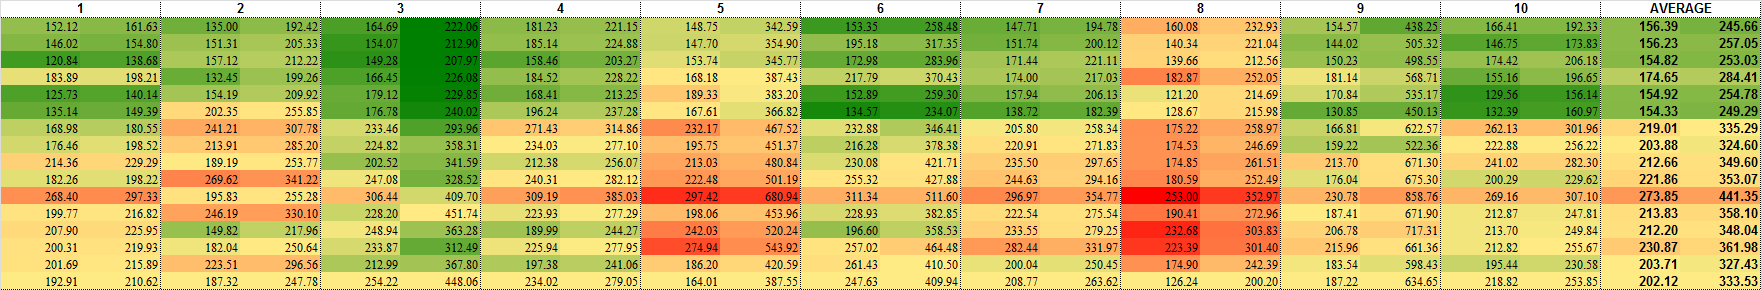
\includegraphics[width=\textwidth]{resultados/p8_percha.png}
	\caption{Routing \emph{scope} 8}
	\label{perchap8}
\end{figure}

\begin{figure}
	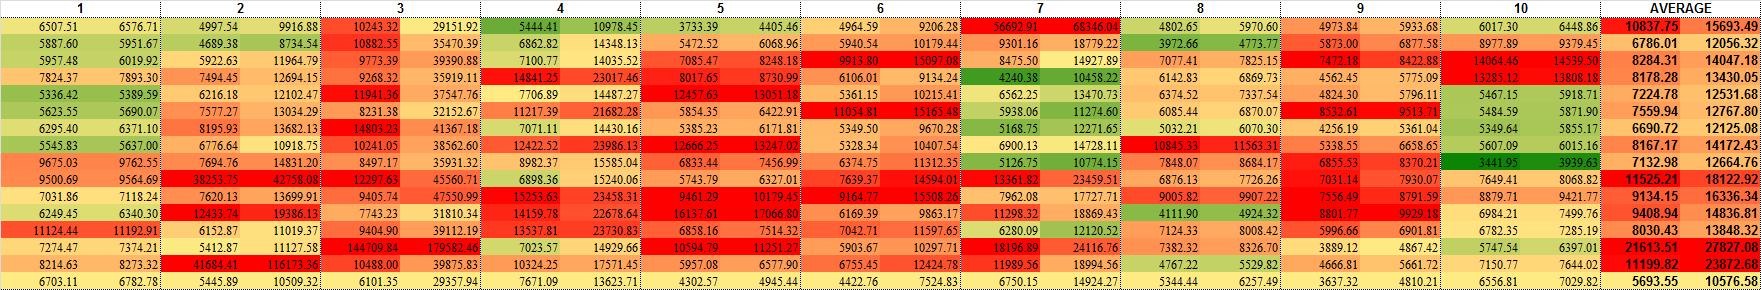
\includegraphics[width=\textwidth]{resultados/p9_percha.png}
	\caption{Routing \emph{scope} 9}
\end{figure}

\begin{figure}
	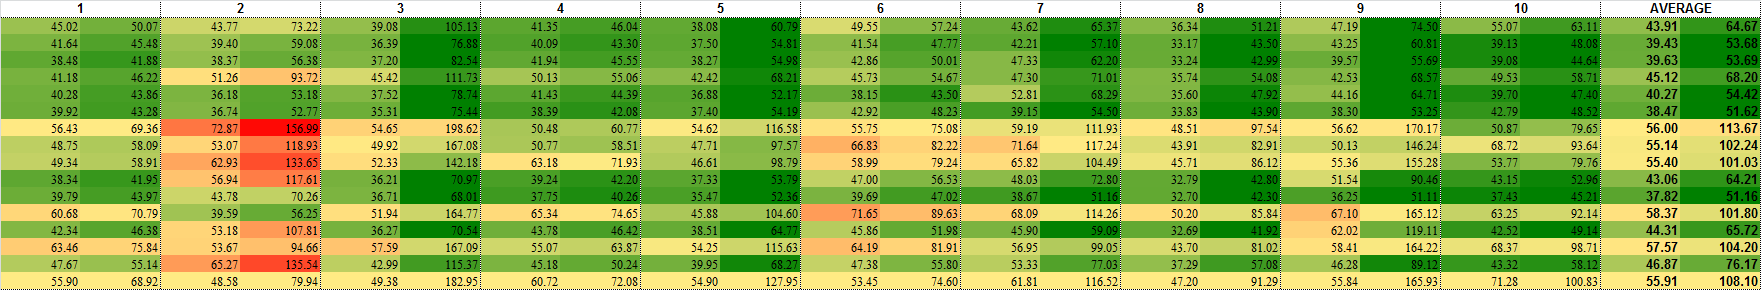
\includegraphics[width=\textwidth]{resultados/k9_percha.png}
	\caption{Closure \emph{scope} 9}
\end{figure}

\begin{figure}
	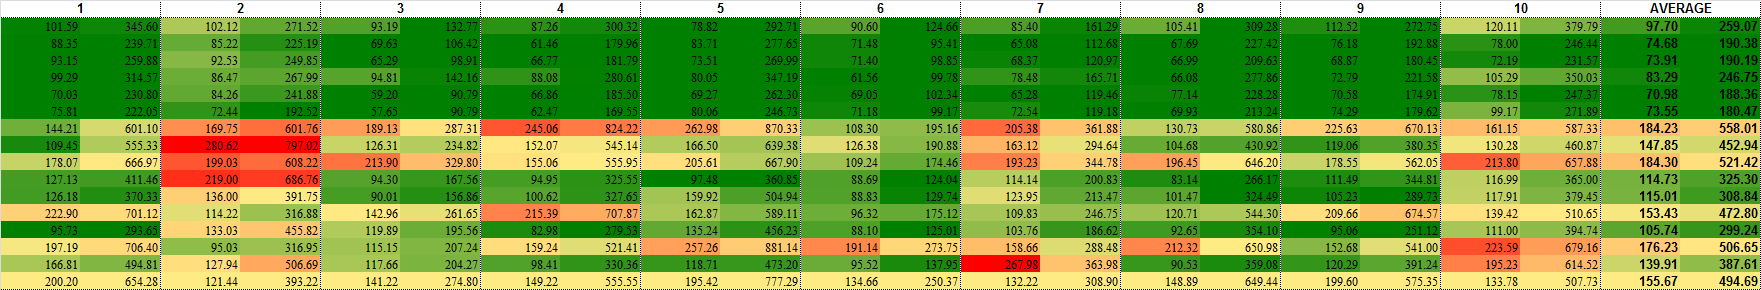
\includegraphics[width=\textwidth]{resultados/k10_percha.png}
	\caption{Closure \emph{scope} 10}
\end{figure}

\begin{figure}
	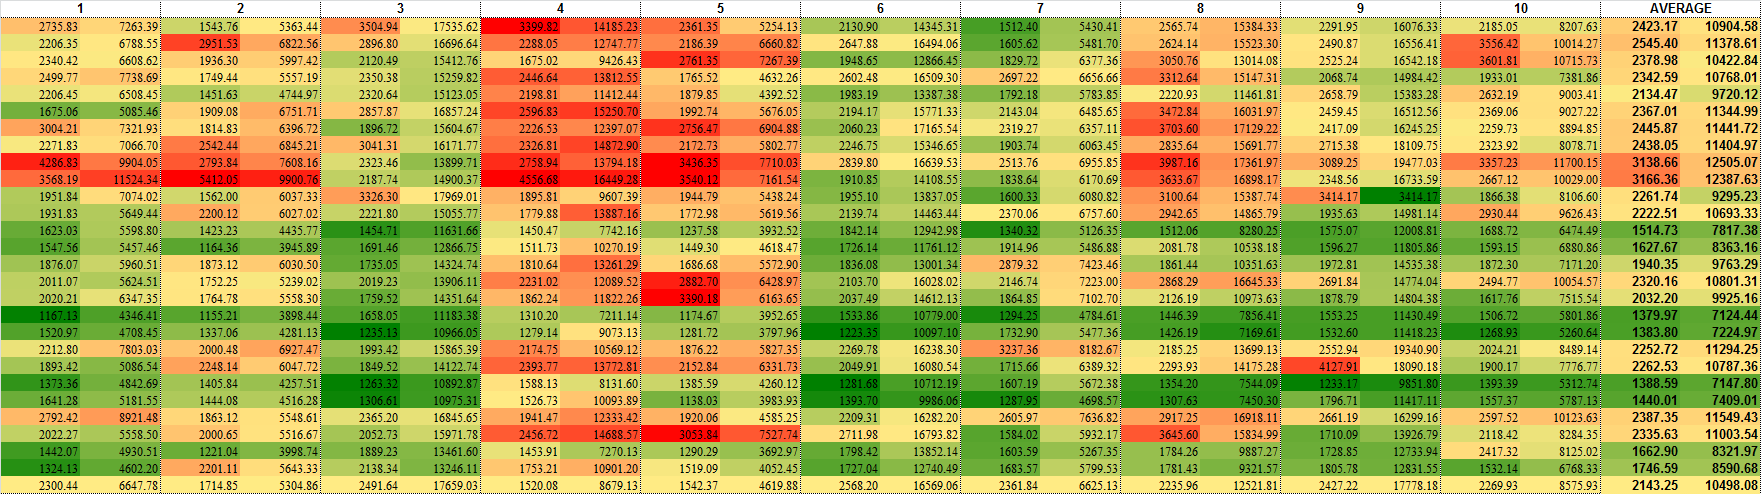
\includegraphics[width=\textwidth]{resultados/soundness8_percha.png}
	\caption{Soundness2 \emph{scope} 8}
	\label{perchasound8}
\end{figure}

Como se puede observar en las figuras, los resultados obtenidos varían de
acuerdo a cada uno de los problemas. Sin embargo es de notar que en la mayoría
de los problemas podemos encontrar uno o varios criterios que reportan
resultados positivos.

Estos resultados no son concluyentes. Esto se debe a que fueron obtenidos en
experimentos en los que el problema fue partido una única vez. En cambio
nuestro enfoque incluye la partición recursiva de un problema. Sin embargo,
entendemos que se los puede considerar como evidencia suficientemente
alentadora como para embarcarnos en la implementación real de esta técnica en
el marco de nuestra herramienta.

\section{Resultados experimentales}

En esta sección mostraremos los resultados experimentales obtenidos a partir
de la implementación de la herencia de cláusulas aprendidas.

Comenzaremos por definir los criterios de selección de cláusulas utilizados.
Cabe aclarar que de aquí en más se considerará que una cláusula aprendida
contiene al menos $2$ literales. Llamaremos \emph{hechos} a las cláusulas de
tamaño $1$.

\subsection{Criterios de selección de cláusulas}

Se probaron tres tipos de criterios:

\begin{itemize}
	\item Por tamaño: Este criterio refiere a la cantidad de literales intervinientes en una cláusula. La motivación de este criterio surge de la observación de que, cuanto más pequeña sea una cláusula, mayor será la porción del árbol de búsqueda que recorte. Recordemos que, en el contexto de nuestro problema, las cláusulas son disyuciones. Por lo tanto una cláusula que contiene $n$ literales nos evita recorrer una $\frac{1}{2^n}$ parte del espacio de búsqueda. Esto se debe a que, de las $2^n$ valuaciones posibles restringidas a los $n$ literales intervinientes, hay una de ellas --en particular aquella que hace que dicha cláusula sea falsa-- que es descartada gracias a la existencia de esta cláusula aprendida. Por lo tanto ninguna valuación que contenga dicha valuación restringida será viable. Por ende, a menor tamaño de cláusula, mayor será el espacio de búsqueda recortado.

	\item Por actividad: En \ref{sec:longactlbd} se explicó a qué nos referimos por actividad de una cláusula. De ello se desprende que la actividad de una cláusula es un indicador de cuántas veces esa cláusula fue (parcialmente) responsable de que ocurra un conflicto. Es de esperar entonces que las cláusulas con mayor actividad sean más relevantes para evitar recorrer ciertas porciones del espacio de de búsqueda.

	\item Por \emph{LBD}: También en \ref{sec:longactlbd} introdujimos la noción de \emph{Literals Block Distance}. Elegimos utilizar esta medida porque se han reportado muy buenos resultados en \ssolvers secuenciales utilizando criterios basados en esta medida.
\end{itemize}

\subsubsection{Parámetros}

En el caso de los criterios por tamaño, los mismos se generaron a partir de un
parámetro que indica el máximo tamaño que puede terner una cláusula para ser
admitida en la herencia. En este caso, todas las cláusulas cuyo tamaño sea
menor o igual que el indicado por el parámetro pasarán a formar parte de la
herencia.

Los criterios por \emph{LBD} funcionan de la misma manera que los basados en
tamaño. En este caso las cláusulas admitidas en la herencia serán aquellas
cuyo \emph{LBD} sea menor o igual al correspondiente parámetro.

Los criterios por actividad se generan a partir de tres parámetros. En primer
lugar un parámetro binario que indica si se desean conservar las cláusulas más
activas o las menos activas. En segundo lugar un parámetro que indica qué
porcentaje de las cláusulas aprendidas del padre se desea conservar y por
último un parámetro binario que indica si, además, se deben conservar todas
aquellas cláusulas aprendidas cuyo tamaño sea 2 (cláusulas binarias).

La incorporación de las cláusulas binarias en los criterios por actividad
surge del hecho de que, el \ssolver secuencial utilizado recorta su base de
datos de claúsulas aprendidas de acuerdo a la actividad pero nunca descarta
las cláusulas binarias.

Además de los tipos de criterios mencionados también se implementó la
posibilidad de heredar los \emph{hechos} aprendidos (o \emph{facts}). La
herencia de los \emph{facts} se implementó de manera tal que pudiera tanto ser
combinada con los distintos tipos de criterios como también utilizada de forma
exclusiva como criterio de herencia.




\subsection{Resultados obtenidos}

\subsubsection{Garping del mejor criterio para cada problema}


\begin{sidewaystable}
	\small
	\begin{tabular}{lrrrrrrrrrr}
		\toprule
		problem	&			&	seq. 				&	reps.	& avg. par.		&	speedup	&	effic.		& best. par.	& best 		& best			& efficiency \\
				&			&		walltime (s)	&	 		& walltime	&			&	 			& walltime		& speedup 	& effic.	& multiplier \\
		\cmidrule(r){1-11}
		Routing	&	8		&	308.26				&		7 	& 60.46			& 5.10x		&	0.08 		& 60.46			&	5.10x	& 0.08			& 1.00
\\
		Routing	&	9		&	76168.16			&	6 		& 407.34		& 	186.99x	&	2.92 		& 387.44		& 196.60x	& 3.07			& 1.05
\\
		Routing	&	$^*$10	&	$>$1209600.00		&	5 		& 5046.84		&$>$239.67x	&	$>$3.74 	& 3213.59		& $>$376.40x	& $>$5.88			& $>$1.57
\\
		\cmidrule(r){1-11}
		Closure	&	11		&	749.65				&	14 		& 291.28		&	2.57x	&	0.04 		& 150.30		&  4.99x	& 0.08			& 1.94
\\		Closure	&	12		&	3983.36				&	5 		& 1914.45		&	2.08x	&	0.03 		& 266.68		& 14.94x	& 0.23			& 7.35
\\		Closure	&	13		&	16261.35			& 5 		&	4362.61		&	3.73x	&	0.06 		& 645.44		& 25.19x	& 0.39			& 6.76
\\
		\cmidrule(r){1-11}
		GC Sound.&	9	&	217.31				&	10 		& 200.85		&	1.08x	&	0.02 		& 168.04		& 1.29x		& 0.02			& 1.20
\\
		GC Sound.&	10	&	 2855.30			&	7 		& 1376.89		&	2.07x	&	0.03 		& 592.54		& 4.82x		& 0.08			& 2.32
\\
		\cmidrule(r){1-11}
		GC Compl.	& 8	&	180.25				&	7 		& 61.50			&	2.93x	&	0.05 		& 36.43			& 4.95x		& 0.08			& 1.69
\\
		GC Compl.	& 9	&	18643.06			&	5 		& 1825.60		&	10.21x	&	0.16 		& 390.48		& 47.74x	& 0.75			& 4.68
\\
		\bottomrule
		\\
		\multicolumn{10}{l}{\begin{tiny}$^*$: Se ejecutó por 14 días sin que el \ssolver secuencial consiga un resultado\end{tiny}}
	\end{tabular}
	\caption{Tiempo de ejecución (en segundos) distribuido vs. secuencial}
	\label{tab:mejorlearning}
\end{sidewaystable}

\subsubsection{Promedios por cada criterio}

\hspace{-5em}
\begin{minipage}{\textwidth}
	\small
	\begin{tabular}{lrrr}
		\toprule
		criteria	&	worst speedup (x)	&	best speedup (x)	&	avg speedup (x) \\
		\cmidrule(r){1-4}
		lbdle2.+facts	&	0.68	&	4.91	&	1.97 \\
		lbdle2.-facts	&	0.71	&	3.84	&	1.24 \\
		lbdle3.+facts	&	0.78	&	5.16	&	1.41 \\
		lbdle3.-facts	&	0.75	&	5.71	&	1.69 \\
		lbdle4.+facts	&	0.64	&	6.80	&	1.68 \\
		lbdle4.-facts	&	0.79	&	5.83	&	1.83 \\
		lbdle5.+facts	&	0.69	&	6.74	&	1.64 \\
		lbdle5.-facts	&	0.77	&	5.25	&	2.14 \\
		lbdle6.+facts	&	0.76	&	5.79	&	1.95 \\
		lbdle6.-facts	&	0.70	&	6.08	&	1.94 \\
		\cmidrule(r){1-4}
		onlyfacts	&	\cellcolor{green}0.84	&	3.23	&	1.45 \\
		\cmidrule(r){1-4}
		perc=0.01.+facts.+binary.+active	&	\cellcolor{red}0.55	&	3.83	&	2.12 \\
		perc=0.01.+facts.+binary.-active	&	0.77	&	3.78	&	1.92 \\
		perc=0.01.+facts.-binary.+active	&	0.64	&	3.64	&	\cellcolor{red}1.19 \\
		perc=0.01.+facts.-binary.-active	&	0.65	&	3.50	&	1.39 \\
		perc=0.01.-facts.+binary.+active	&	0.74	&	2.73	&	1.91 \\
		perc=0.01.-facts.+binary.-active	&	0.69	&	2.38	&	1.30 \\
		perc=0.01.-facts.-binary.+active	&	0.74	&	\cellcolor{red}1.68	&	1.22 \\
		perc=0.01.-facts.-binary.-active	&	0.71	&	2.22	&	1.22 \\
		\cmidrule(r){1-4}
		sizele2.+facts	&	0.75	&	3.50	&	1.57 \\
		sizele2.-facts	&	0.81	&	3.32	&	\cellcolor{red}1.19 \\
		sizele3.+facts	&	\cellcolor{red}0.55	&	5.40	&	1.63 \\
		sizele3.-facts	&	0.75	&	3.87	&	1.39 \\
		sizele4.+facts	&	0.74	&	6.24	&	1.91 \\
		sizele4.-facts	&	0.72	&	4.21	&	1.81 \\
		sizele5.+facts	&	0.64	&	6.14	&	1.92 \\
		sizele5.-facts	&	0.58	&	\cellcolor{green}7.18	&	1.90 \\
		sizele6.+facts	&	0.72	&	5.08	&	2.17 \\
		sizele6.-facts	&	0.79	&	5.69	&	\cellcolor{green}2.61 \\
		\bottomrule
	\end{tabular}
	%\caption{Tiempo de ejecución (en segundos) distribuido vs. secuencial}
\end{minipage}

\subsubsection{Heatmaps para scopes crecientes}


\subsection{Discusión y conclusiones}
